In this section the individual components will be discussed in terms of the needed high level sub-parts and their functioning, as well as how those sub-elements interface with one another within the overlaying component and which of them is in charge of interfacing with other components.

\subsection{Database}
The database layer must include a DBMS component, in order to manage the insertion, modification, deletion and logging of transactions on data inside the storage memory.

Regardless of the implementation, the DBMS must guarantee the correct functioning of concurrent transactions and the ACID properties; it also must be a relational DBMS, since the application needs in terms of data storage do not require a more complex structure than the simple one provided by the relational data structure.

The data layer must only be accessible through the Application Server via a dedicated interface. With respect to this, the Application Server must provide a persistence unit to handle the dynamic behaviour of all of the persistent application data.

The Database must be tuned during the implementation phase in order to ensure security by granting data access according to the privilege level of the requester. Sensible data such as passwords and personal information must be encrypted properly before being stored. Users must be granted access only upon provision of correct and valid credentials.

The E-R diagram in Figure \ref{er_dg} illustrates a concept of the Database schema.

\begin{figure}[H]
\begin{center}
		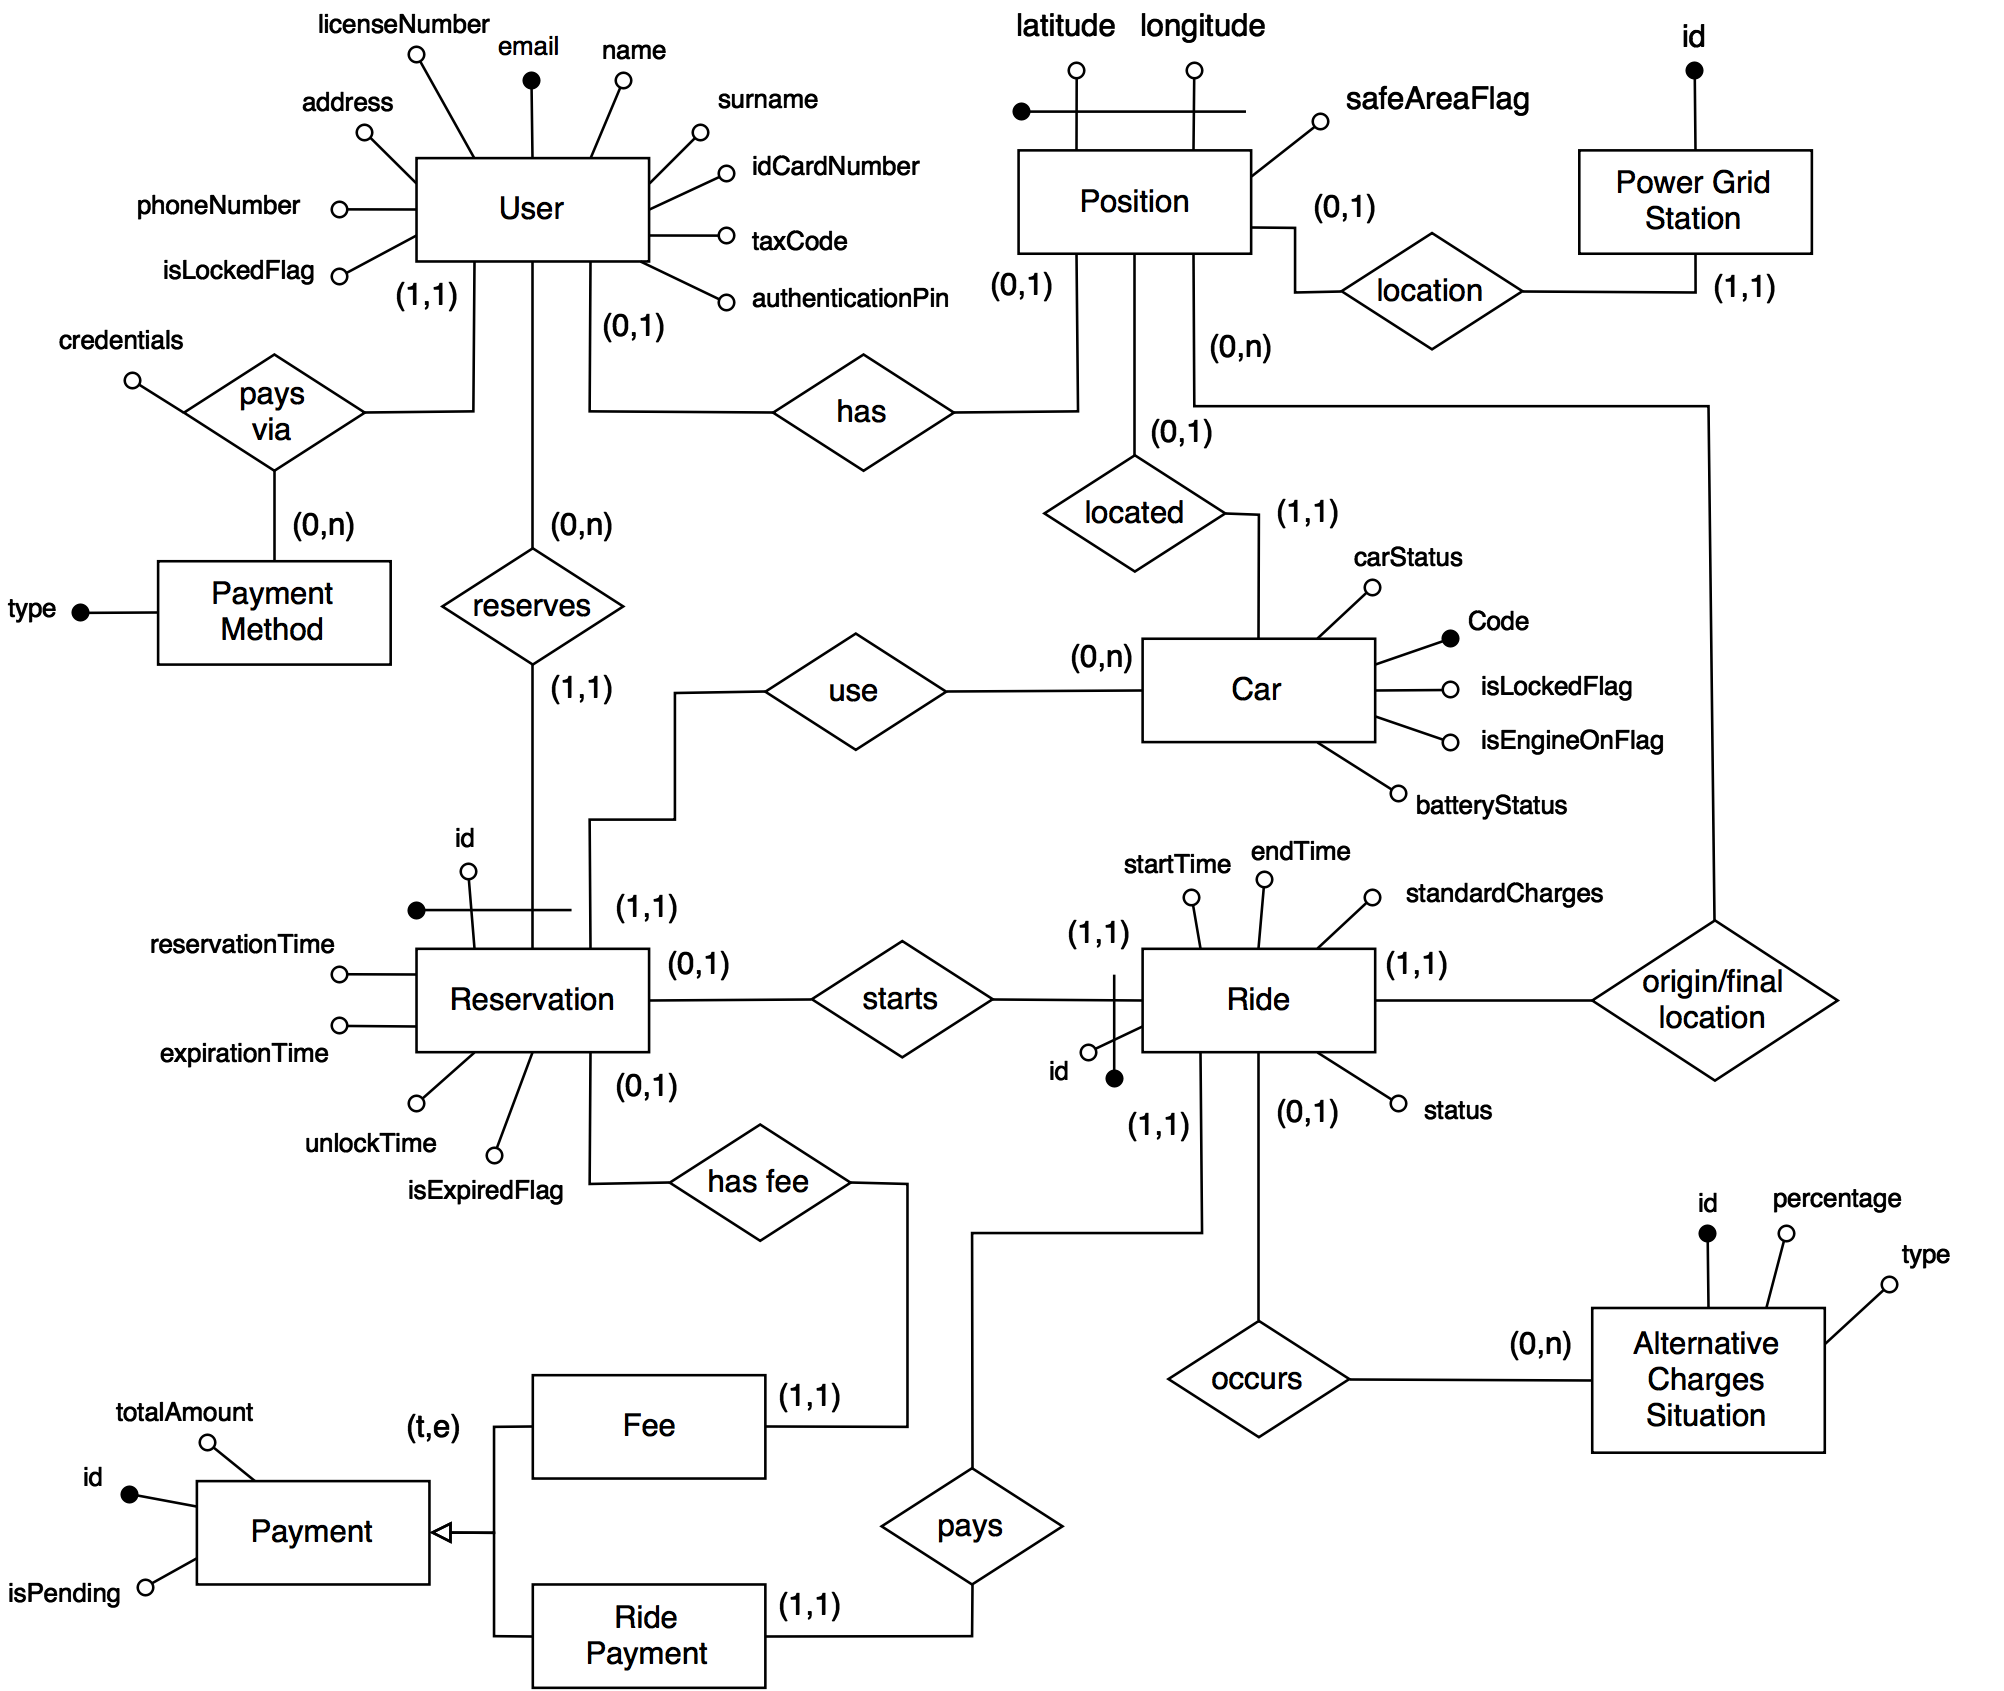
\includegraphics[width=0.9\textwidth]{./arch_design/diagrams/er_dg.png}
		\caption{The E-R diagram of the database schema. Note that the relation named "origin/final location" must be considered as a short-hand notation to indicate two distinct relations: one for the starting location of the ride and one for the ending location.}
		\label{er_dg}
\end{center}
\end{figure}

\subsection{Application Server}
This layer must handle the business logic as a whole and the connections with the data layer and the multiple ways of accessing the application.

The main feature of the Application Server are the specific modules of business logic, which describe business rules and work-flows for each of the functionalities provided by the application itself.

The interface with the data layer must be handled, as stated in the previous section, by a dedicated persistence unit, that will be in charge of the object-relation mapping and dynamic data access and management; this ensures the fact that only the Application Server can access the Database.

The Application Server must provide a means to interface with the Web Server and the mobile and on-board clients via specific APIs in order to decouple the different layers with respect to their individual implementation. Moreover, it must provide a way to communicate with external systems by adapting the application to the existing external infrastructures.

The main business logic modules must include:

\begin{description}
\item[UserManager:] This module will manage all the logic involved with user account management, login, registration, profile customization and management, as well as the generation and provision of user credentials.
\item[ReservationManager:] This module provides the logic behind the reservation management, with particular focus on the timing restrictions, car status updates (via the CarStatusManager) and reservation release conditions. It is also in charge of the controls to be performed in order to avoid multiple reservations by a user; lastly it must handle concurrent reservation issues such as pseudo-simultaneous requests for the same car.
\item[RideManager:] The logic included in this module is in charge of record all useful information about the rides as provided by the on-board application, including ride time, car battery levels and ride charges. It also manages the ride status updates.
\item[MapManager:] This module contains the logic used to locate cars and users, as well as defining the Safe Area boundaries and the power grids locations. It must provide useful data to the ReservationManager and the RideManager logic units, since both of them need localization information to perform their functionalities.
\item[CarStatusManager:] This module includes the logic needed by other components to set the car status of a car. It must also serve as an interface with the external maintenance system by providing an automatic way to signal out-of-service cars.
\item[SecurityAuthenticator:] All the logic in charge of performing user-reservation-car matches is included in this module: this includes the control over cars unlocking and the logic behind the on-board authentication method.
\item[DiscountProvider:] This module is in charge of recording virtuous and bad situations as parameters of rides, so that the PaymentGateway can gather all the needed information to compute the corresponding net total charges.
\item[PaymentGateway:] The logic involved in the computation of final charges is included in this module; moreover, this unit must stand as an interface with the payment handlers upon the act of the automatic payments.
\item[NotificationManager:] Serves as a gateway from all the modules that need to notify the client towards the clients themselves by managing the logic behind the notifications services.
\end{description}

\subsection{Web Server} %specificare perché non c'è il browser nell'elenco
The Web Server layer is the interface between clients and the business logic layer in case the access to the application services is performed via web browser.

That being said, it is clear that the main functions to be implemented by this layer will essentially consist of interfaces, since - as stated in Section \ref{high_level_comps} - there will not be any logic implemented within the Web Server besides the presentation of pages.

The presentation must be structured in a clean and simple way, such that the components providing the client with web pages are decoupled as possible from the components that interface with the business logic subsiding the Application Server in order to fetch relevant data to be shown.

Adequate APIs must be designed in order to separate in the most efficient way the design of the Web and Application Servers. These APIs must be thought in a way that allows quick and efficient data transfer through textual data files over HTTPS, e.g. XML or JSON.

The interface with web browsers must be performed efficiently and following similar design concepts.

\subsection{Mobile Application Client}
The Mobile Client must be designed in a way that makes communications with the Application Server easy and independent from the implementation of both sides.

In order to do so, adequate APIs must be defined and used similarly to what has been described for the interactions between the two server layers.

The mobile application must be designed following the guidelines provided by the Android and iOS producers. More detail on which packages and languages to be used will be put in Section \ref{impl_choices}.

\subsection{On-Board Application Client}
The On-Board Application consists of an application designed to run on pre-existing embedded devices on every car. The devices come together with the rest of the car equipment directly from the manufacturer.

For this reason, the application must be designed following the guidelines provided by the manufacturer and based on given APIs.

As far as the interface with the Application Server, the same considerations made with respect to the mobile application must be taken into account also for the on-board application.

%insert global component view diagram: show high-level comps and interfaces

%PARAGRAPH: IMPLEMENTATION CHOICES\label{impl_choices}
%we specify the JEE choice and we put all EJB and shit pictures and diagrams
%also all specifications not in RASD